\PassOptionsToPackage{subsection=false}{beamerouterthememiniframes}
\documentclass{beamer}

\usetheme{Szeged}
%\usepackage{pgfpages}
%\setbeameroption{show notes on second screen=right}
\setbeamertemplate{navigation symbols}{}
%\usecolortheme[named=black]{structure}
\definecolor{db}{HTML}{3A4454}
\definecolor{elblue}{HTML}{53687e}
\setbeamercolor{palette primary}{bg=blue,fg=white}
\setbeamercolor{palette secondary}{bg=blue,fg=white}
\setbeamercolor{palette tertiary}{bg=elblue,fg=white}
\setbeamercolor{palette quaternary}{bg=black,fg=white}
\setbeamercolor{structure}{fg=db} % itemize, enumerate, etc
\setbeamercolor{section in toc}{fg=black} % TOC sections
\setbeamercolor{frametitle}{bg=white,fg=elblue}
% Override palette coloring with secondary
\setbeamercolor{subsection in head/foot}{bg=gray,fg=white}

\setbeamertemplate{section in toc}{\inserttocsectionnumber.~\inserttocsection}

\usepackage{xurl}
\usepackage{amsmath,amsfonts}
\usepackage[backend=biber]{biblatex}
\addbibresource{presentation/bibliography.bib}
\usepackage{tikz}
\usetikzlibrary{shapes.geometric, arrows, positioning, arrows.meta}
\usepackage{mathrsfs}
\usefonttheme[onlymath]{serif}
\usepackage{graphicx}

\newcommand{\R}{\mathbb{R}}
\newcommand{\E}{\mathbb{E}}
\newcommand\dint{\mathord{\mathrm{d}}}
\newcommand{\M}{\mathbf{M}}
\newcommand{\A}{\mathbf{A}}
\newcommand{\B}{\mathbf{B}}

\begin{document}

\title{Charakteristische Funktionen}
%\subtitle{}
\author{Maximilian Ernst}
\date{\today}
\begin{frame}
\titlepage
\end{frame}

\begin{frame}\frametitle{Inhalt}\tableofcontents\end{frame}

%%%%%%%%%%%%%%%%%%%%%%%%%%%%%%%%%%%%
\section{Motivation}
%%%%%%%%%%%%%%%%%%%%%%%%%%%%%%%%%%%%
\begin{frame}
\frametitle{Versicherungen}
Wie viele Schadensmeldungen erhält eine Versicherung in einem Zeitintervall $(0, t)$?\\
\hfill \newline

\only<1>{
\begin{itemize}
    \item[--] Wir zerlegen das Intervall in $n$ Teilintervalle der Länge $\frac{t}{n}$
    \item[--] n groß $\to$ Teilintervalle kurz $\to$ Annahme, dass nur ein Schaden auftritt
    \item[--] in einem Intervall kann also ein Schaden auftreten oder kein Schaden (mit Wahrscheinlichkeit $p$)
    \item[--] $p = \alpha \frac{t}{n}$
    \item[--] Die einzelnen Teilintervalle sind unabhängig
\end{itemize}
}

\only<2>{
Das bedeutet: eine "Unglücksfee" zieht n mal eine "Kugel" auf der steht "Schaden" (mit Wahrscheinlichkeit $p$) oder "kein Schaden" (mit Wahrscheinlichkeit $1-p$), mit $p = \alpha \frac{t}{n}$.

Anzahl der Schadensfälle $k \sim Bin_{n, \alpha \frac{t}{n}}$

Je größer wir n wählen, desto besser die Approximation. Also:

$$P(k) = \lim_{n \to \infty} Bin_{n, \alpha \frac{t}{n}}$$
}
\end{frame}

\begin{frame}
\frametitle{Versicherungen}
Sei $p_n$ eine Folge von Wahrscheinlichkeiten mit $n p_n \to \lambda$. Dann gilt:

$$\lim_{n \to \infty} Bin_{n, p_n}(k) = Poiss_\lambda (k)$$
\end{frame}

\begin{frame}[fragile]
\frametitle{Versicherungen}
{\footnotesize
  \begin{align*}
 \textcolor<2>{red}{{n \choose k}} p_n^k(1-p_n)^{n-k} &= \textcolor<2>{red}{\frac{n!}{k!(n-k)!}} p_n^k(1-p_n)^{n-k}\\
  &= \frac{\textcolor<3>{red}{n^k}}{k!} \textcolor<4>{red}{\frac{n!}{\textcolor<3>{red}{n^k}(n-k)!}} p_n^k(1-p_n)^{\textcolor<4>{red}{n-k}}\\
  \; &\sim \frac{\textcolor<5>{red}{n^k}}{k!} \textcolor<5>{red}{p_n^k}(1-p_n)^{\textcolor<4>{red}{n}}\\
  &= \frac{\textcolor<5>{red}{(np_n)^k}}{k!}(1-p_n)^n\\
  &= \frac{(\textcolor<7>{red}{np_n})^k}{k!}\Big(1-\frac{\textcolor<7>{red}{\textcolor<6>{red}{n}p_n}}{\textcolor<6>{red}{n}}\Big)^n\\
  &\sim \frac{\textcolor<7>{red}{\lambda}^k}{k!}\textcolor<8>{red}{\Big(1-\frac{\textcolor<7>{red}{\lambda}}{n}\Big)^n}\\
  \only<8>{\textcolor{blue}{\tiny{\Bigg(1 + \frac{x}{n} \Bigg)^n \to e^x}} \hspace{5pt}} &\to \frac{\lambda^k}{k!}\textcolor<8>{red}{e^{-\lambda}}\\
  \end{align*}
}%
\end{frame}

\begin{frame}
$$\text{Geht das auch einfacher?} \to \text{Ja!}$$
\end{frame}

\begin{frame}
\frametitle{Ziel}
Jeder (reellwertigen) Zufallsvariable ein möglichst "einfaches" mathematisches "Objekt" zuordnen, sodass wir Berechnungen und Beweise mit diesem Objekt (statt der Zufallsvariable) machen.
\hfill \newline
\begin{itemize}
    \item[--] Verteilung der Summe unabhängiger Zufallsvariablen
    \item[--] Berechnung von Momenten
    \item[--] Beweis von Verteilungskonvergenzen
\end{itemize}
\end{frame}


\begin{frame}
\frametitle{Dualität}
\textit{Manchmal bilden sehr unterschiedliche mathematische Objekte nur zwei Seiten der selben Medaille}
\end{frame}

\begin{frame}
\frametitle{Beispiel 1 - Flächeninhalt von Kreisen}
Betrachte die Menge aller Kreise.

Die duale Menge ist die Menge aller einbeschriebenen Quadrate.\\
\hfill \newline
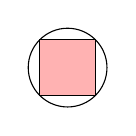
\begin{tikzpicture}
\node (start) [circle, minimum width=1cm, minimum height=1cm, text centered, draw=black] {};
\node (end) [rectangle, minimum width=0.7061cm, minimum height=0.7061cm, text centered, draw=black, fill=red!30] {};
\end{tikzpicture}\\
\hfill \newline
Die Relation $>$ für den Flächeninhalt bleibt erhalten.
\end{frame}

\begin{frame}
\frametitle{Beispiel 2 - Berechnung von Produkten}

$$\ln xy = \ln x + \ln y $$
$$xy = \exp(\log xy) = \exp(\log x + \log y)$$\\
\hfill \newline
Zur Berechnung großer Produkte:
\begin{itemize}
    \item[--] Berechne den Logarithmus
    \item[--] addiere das Ergebnis
    \item[--] nimm $\exp$ des Ergebnisses
\end{itemize}
\end{frame}

\begin{frame}
\frametitle{Beispiel 2 - Berechnung von Produkten}
{\footnotesize
\begin{align*}
L(x_1, \dots, x_n|\mu, \Sigma) &= \prod_{i = 1}^{n} L(x_i|\mu, \Sigma)\\
&= \prod_{i = 1}^{n} (2 \pi)^{-d/2} \det(\Sigma)^{-1/2} \exp(- \frac{1}{2} (x_i - \mu)^T \Sigma^{-1} (x_i - \mu))
\end{align*}

\begin{align*}
\log L(x_1, \dots, x_n|\mu, \Sigma) &= \sum_{i = 1}^{n} \log L(x_i|\mu, \Sigma)\\
&= \sum_{i = 1}^{n} -\frac{d}{2} \log 2\pi -\frac{1}{2} \log \det(\Sigma) - \frac{1}{2} (x_i - \mu)^T \Sigma^{-1} (x_i - \mu)
\end{align*}

}%


\end{frame}

%%%%%%%%%%%%%%%%%%%%%%%%%%%%%%%%%%%%
\section{Definition}
%%%%%%%%%%%%%%%%%%%%%%%%%%%%%%%%%%%%

\begin{frame}
\frametitle{Definition}
Für eine Zufallsvariable X mit Werten in $\R$ bezeichnet
\begin{align*} \label{eq1}
\varphi^X(u) &= \E[e^{iuX}] \only<2->{\\
  & = \int_{\R} e^{iux} \dint P^X(x)} \only<3>{\\
 & = \int_{\R} \cos(ux) \dint P^X(x) + i \int_{\R} \sin(ux) \dint P^X(x)}
\end{align*}

ihre charakteristische Funktion.

\end{frame}

\begin{frame}
\frametitle{Beispiel 1 - Normalverteilung}
Sei $X \sim N(0,1)$. Dann ist die Dichte
{\footnotesize
$$ f_X(x) = \frac{1}{\sqrt{2 \pi}} e^{-\frac{x^2}{2}} $$
}%
Also ist
{\footnotesize
\begin{align*}
\varphi_X(u) &= \E[e^{iuX}]\\
&= \int_\R e^{iux}f_X(x) \dint x\\
&= \int_\R e^{iux} \frac{1}{\sqrt{2 \pi}} e^{-\frac{x^2}{2}}\\
&= e^{-\frac{u^2}{2}}
\end{align*}
}%
\end{frame}

\begin{frame}
\frametitle{Beispiel 1 - Normalverteilung}
\includegraphics[width=\linewidth, height=\textheight,keepaspectratio]{presentation/plots/normal_char.pdf}
\end{frame}

\begin{frame}
\frametitle{Eigenschaften}
$\varphi$ sollte besonders "einfach" sein
\hfill \newline
\begin{itemize}
    \setlength\itemsep{1em}
    \item[--] $\varphi(0) = 1$
    \item[--] $|\varphi| \leq 1$
    \item[--] gleichmäßig stetig
\end{itemize}
\end{frame}

\begin{frame}
\frametitle{Beispiel 2 - $\varphi$ ist "einfach"}
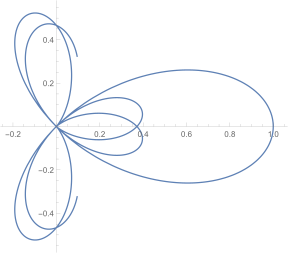
\includegraphics[width=\linewidth, height=\textheight,keepaspectratio]{presentation/plots/cantor.pdf}
\end{frame}

\begin{frame}
\frametitle{Beispiel 2 - $\varphi$ ist "einfach"}
\includegraphics[width=\linewidth, height=.4\textheight,keepaspectratio]{presentation/plots/cantor_re.pdf}
\includegraphics[width=\linewidth, height=.4\textheight,keepaspectratio]{presentation/plots/cantor_im.pdf}
\end{frame}

%%%%%%%%%%%%%%%%%%%%%%%%%%%%%%%%%%%%
\section{Anwendung}
%%%%%%%%%%%%%%%%%%%%%%%%%%%%%%%%%%%%

\begin{frame}
\frametitle{Faltung - Dichten}
  Seien $X, Y$ unabhängige reellwertige ZV die beide eine Dichte $f^X, f^Y$ besitzen. Dann besitzt $X+Y$ die Dichte

\begin{equation*}
  f^{X+Y}(z) = \int_{\R} f^X(z - y)f^Y(y) \dint y, \; z \in \R
\end{equation*}

(eng.: convolution)
\end{frame}

\begin{frame}
\frametitle{Faltung - Beispiel}
Seien $X \sim Gamma(\lambda, p_1)$ und $Y \sim Gamma(\lambda, p_1)$ unabhängig. Die Dichte der Gamma-Funktion ist

$$f_{\lambda, p}(x) = \frac{\lambda^p}{\Gamma(p)} x^{p-1} e^{-\lambda x} \mathbf{1}_{(0, \infty)} (x)$$

Es ergibt sich also für die Faltung
{\scriptsize
$$f^{X+Y}(z) = \int_\R \frac{\lambda^{p_1}}{\Gamma(p_1)} (z-y)^{p_1-1} e^{-\lambda (z-y)} \mathbf{1}_{(0, \infty)} (z-y) \frac{\lambda^{p_2}}{\Gamma(p_2)} (y)^{p_2-1} e^{-\lambda (y)} \mathbf{1}_{(0, \infty)} (y) \dint y$$
}%
\end{frame}

\begin{frame}
\frametitle{Faltung - CF}
  Seien $X, Y$ unabhängige reellwertige ZV mit charakteristischen Funktionen $\varphi^X, \varphi^Y$. Dann besitzt $X + Y$ die charakteristische Funktion
$$\varphi^{X+Y} = \varphi^X \varphi^Y$$
\end{frame}

\begin{frame}
\frametitle{Faltung - Beispiel}
Seien $X \sim Gamma(\lambda, p_1)$ und $Y \sim Gamma(\lambda, p_1)$ unabhängig. Die charakteristische Funktion ist

$$\varphi^{Gamma(\lambda, p)}(u) = \Bigg(1-\frac{u}{\lambda}\Bigg)^{-p}$$

Es ergibt sich also für die Faltung
{\tiny
$$\varphi^{X+Y}(u) = \varphi^{X}(u)\varphi^{Y}(u) = \Bigg(1-\frac{u}{\lambda}\Bigg)^{-p_1} \Bigg(1-\frac{u}{\lambda}\Bigg)^{-p_2} = \Bigg(1-\frac{u}{\lambda}\Bigg)^{-(p_1+p_2)} = \varphi^{Gamma(\lambda, p_1 + p_2)}(u)$$
}%
\end{frame}

\begin{frame}
\frametitle{Momente}
Besitzt die ZV $X \; p$ endliche Momente, ist $\varphi^X \; p$-mal stetig differenzierbar und es gilt für $k < p$

\begin{equation*}
\E[X^k] = \frac{(\varphi^X)^{(k)}(0)}{i}
\end{equation*}
\end{frame}

\begin{frame}
\frametitle{Momente - Beispiel}
Sei $X \sim N(\mu, \sigma^2)$. Gesucht: $\E[X]$.

Es ist

$$\E[X] = \frac{\varphi_X^{(1)}(0)}{i}$$
\end{frame}

\begin{frame}
\frametitle{Momente - Beispiel}
Wir berechnen

$$\frac{\dint}{\dint u} \varphi_X = \frac{\dint}{\dint u} \exp(i \mu u - \frac{1}{2} \sigma^2 u^2) = \exp(i \mu u - \frac{1}{2} \sigma^2 u^2) (i \mu - \sigma^2 u)$$

Ausgewertet an der Stelle 0

$$\varphi_X^{(1)}(0) = \exp(0 - 0) (i \mu - 0) = 1 \cdot i \mu$$
\end{frame}

\begin{frame}
\frametitle{Momente - Beispiel}
Eingesetzt in unsere Formel

$$\E[X] = \frac{\varphi_X^{(1)}(0)}{i} = \frac{i \mu}{i} = \mu$$
\end{frame}

\begin{frame}
\frametitle{Konvergenz in Verteilung}
\textbf{Stetigkeitssatz von Levy:} \hfill \newline
Seien $P_n$ Wahrscheinlichkeitsmaße auf $(\R, \mathfrak{B}_\R)$ mit charakteristischen Funktionen $\varphi_n$ und gilt $\lim_{n \to \infty} \varphi_n (x) = \varphi(x)$ für alle $x \in \R$ und eine bei $x = 0$ stetige Funktion $\varphi$, so ist $\varphi$ die charakteristische Funktion eines Wahrscheinlichkeitsmaßes $P$ auf $(\R, \mathfrak{B}_\R)$ und es gilt: $P_n \to P$.
\end{frame}

\begin{frame}
\frametitle{Konvergenz in Verteilung - Beispiel}
Wir haben eine Folge von Wahrscheinlichkeitsmaßen $Bin(n, p_n)$ mit $np_n \to \lambda$. Es gilt:

$$\varphi^{Bin(n, p_n)}(u) = (1 + p_n(e^{iu} - 1))^n$$

Wir erhalten also
{\footnotesize
$$\varphi^{Bin(n, p_n)}(u) = (1 + p_n(e^{iu} - 1))^n = \Bigg(1 + \frac{\textcolor{red}{np_n(e^{iu} - 1)}}{n}\Bigg)^n \to e^{\textcolor{red}{\lambda(e^{iu}-1)}} = \varphi^{Poiss(\lambda)}$$
}%
\end{frame}


\begin{frame}
\frametitle{Referenzen}
\nocite{*}
\printbibliography
\end{frame}
\end{document}
